\documentclass[10pt]{article}

% Manuscript v6 (draft, 19 Nov 2026). Honest reporting version: it names the method by what was
% measured (CARE), reports every pre-registered hypothesis including the ones not supported, labels
% post-hoc findings as such, and marks the confirmatory LongMemEval-S run as pending.
\usepackage[letterpaper,margin=1in]{geometry}
\usepackage{times}
\usepackage{amsmath,amssymb,amsthm}
\usepackage{booktabs}
\usepackage{graphicx}
\usepackage{array}
\usepackage{multirow}
\usepackage{xcolor}
\usepackage{float}
\usepackage[round]{natbib}
\usepackage{hyperref}
\hypersetup{colorlinks=true,linkcolor=blue,citecolor=blue,urlcolor=blue}
\emergencystretch=2em

\theoremstyle{plain}
\newtheorem{proposition}{Proposition}
\newtheorem{lemma}{Lemma}
\newtheorem{theorem}{Theorem}
\newtheorem{corollary}{Corollary}

\newcommand{\care}{\textsc{CARE}}
\newcommand{\pending}[1]{\textcolor{red}{\textbf{[PENDING: #1]}}}
\newcommand{\sub}{\sqsubseteq}
\newcommand{\A}{\mathcal{A}}
\newcommand{\F}{\mathcal{F}}

\title{\textbf{\care{}: Conditional Answer Repair with Source-Anchored Evidence\\
for Long-Horizon Conversational Question Answering}}
\author{Anonymous authors\\ \small Draft v6 --- not under review}
\date{}

\begin{document}
\maketitle

\begin{abstract}
A conversational reader must answer questions about histories far longer than its context window. We
study \care{}, a bounded reader over an append-only archive of original turns. It ranks turns with BM25
or dense embeddings, answers with cited turn identifiers that code checks against the visible bundle,
and may repair an abstention once. We evaluate with open models only (Qwen3-8B reader,
Qwen3-Embedding-0.6B encoder) on all 1,986 LoCoMo questions, which we used for development, and on the
500 LongMemEval cleaned-oracle questions, which we used for a confirmatory check. Repair raises the
LoCoMo score from 0.459 to 0.526 and beats a same-reader dense RAG baseline (0.457) by 0.069, but it
reverses 46 correct refusals. Replacing BM25 by a dense first bundle helps before repair
(+0.014, 9 of 10 conversations) and not after it. Adding dense evidence to repair (hybrid repair) gives
the best development score (0.541), but this variant was selected after inspecting development results
and does not reach significance on LongMemEval (+0.005, interval containing zero). Graph-based repair
does not improve on hybrid repair on either benchmark. A repair verifier must catch refusal-losing repairs
at least 3.89 times as often as it rejects useful ones, and six verifiers we built fall below this bound.
We do not claim superiority over published memory systems, and the memory write path is implemented and
unit-tested but not evaluated end to end.
\end{abstract}

% =====================================================================================
\section{Introduction}
\label{sec:intro}

Agents that converse over months must answer questions whose evidence was said long ago, may have
been updated, or belongs to a particular speaker. Memory systems address this by writing structured notes
during the conversation \citep{packer2023memgpt,chhikara2025mem0,amem2025,memoryr12025,cao2026higmem}, or by
keeping the history and selecting evidence per question \citep{du2026memr3,wang2026cuemem,liu2026livectx,chen2026justmem,yu2026lazymem}.
Corrective retrieval reads again when a first answer looks unsupported \citep{jiang2023active,asai2023selfrag,yan2024crag}.

This paper reports a bounded reader, \care{}, and a set of controlled measurements of what helps and what
does not. Our design question is narrow: once original turns are kept and cited, how much does a second
read help, and what does it cost? The answers we find are mixed, and we report them as such.

\paragraph{Contributions.}
\begin{enumerate}
  \item \textbf{A source-anchored bounded reader} (Section~\ref{sec:method}): an append-only archive of
  turns, citation checks against the visible bundle, a gate, and one repair read whose expansion can be
  lexical, dense, or graph-based.
  \item \textbf{A controlled comparison with open models} (Section~\ref{sec:results}): nine systems on the
  same 1,986 LoCoMo questions and a $2\times3$ factorial of first bundle and repair expansion, with
  pre-registered hypotheses, the ones that failed included.
  \item \textbf{A measured cost of repair} (Section~\ref{sec:abstention}): repair converts refusals into
  answers, and we derive and test the condition under which a verifier can recover the lost refusals.
  \item \textbf{A retrieval finding}: with Qwen3-Embedding-0.6B the dense first bundle beats BM25 before
  repair, which reverses an earlier conclusion drawn with a weaker encoder.
\end{enumerate}

\paragraph{What this paper does not claim.} It does not show that the graph memory helps (it does not, in
our measurements), that memory evolution improves accuracy (the write path is not evaluated), or that
\care{} outperforms published memory systems (we did not reproduce them under our reader and metric).

% =====================================================================================
\section{Related Work}
\label{sec:related}

\paragraph{Persistent memory.} MemGPT pages information between context and storage \citep{packer2023memgpt}.
Mem0 extracts and consolidates facts \citep{chhikara2025mem0}; A-Mem links and revises notes \citep{amem2025};
Memory-R1 learns write operations \citep{memoryr12025}; HiGMem maintains an event--turn hierarchy and refreshes
summaries as turns arrive \citep{cao2026higmem}. These systems change what is stored; \care{} keeps the stored
text fixed and changes only how it is read.

\paragraph{Read-time access.} MemR$^3$ routes among retrieval and answering while tracking evidence gaps
\citep{du2026memr3}; CueMem and LiveCtx rebuild context from raw turns \citep{wang2026cuemem,liu2026livectx};
JustMem selects lookup, composition or replay per query \citep{chen2026justmem}; LazyMem builds compact memory
at query time \citep{yu2026lazymem}.

\paragraph{Graph and corrective retrieval.} Personalized PageRank gives local, seed-centred relevance
\citep{andersen2006local}, and HippoRAG applies it to long-term memory \citep{gutierrez2024hipporag}. FLARE,
Self-RAG, Adaptive-RAG and CRAG decide when to retrieve again \citep{jiang2023active,asai2023selfrag,jeong2024adaptive,yan2024crag}.

% =====================================================================================
\section{Method: \care{}}
\label{sec:method}

\begin{figure}[t]
\centering
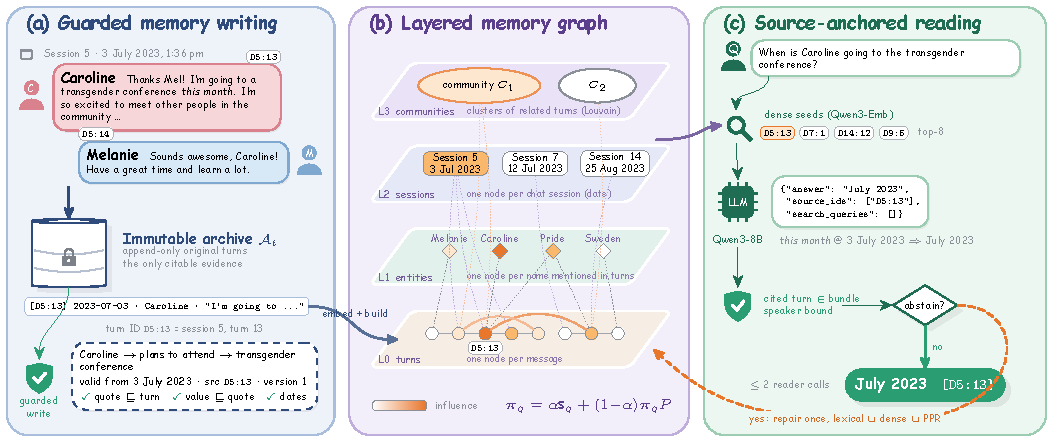
\includegraphics[width=\linewidth]{figures/asem_method_figure.pdf}
\caption{Overview of the system as evaluated. \textbf{(a)} Original turns enter an append-only archive, the only citable
evidence; the write path (guarded operators) is implemented but not part of any reported result. \textbf{(b)} The
layered memory graph is built per conversation without an LLM and is an exploratory component: it did not improve
the score. \textbf{(c)} The reader answers from a top-8 first bundle with cited identifiers, code checks bind the citations
to the bundle, and an abstention with searches triggers at most one repair. The example is a saved output of our run
(LoCoMo \texttt{conv-26}, question 17); node shading in (b) illustrates the mechanism.}
\label{fig:overview}
\end{figure}

\subsection{Archive and first bundle}

A conversation is a stream of turns $s_i=(\mathrm{id}_i,\sigma_i,t_i,p_i,x_i)$ with session $\sigma_i$, date
$t_i$, speaker $p_i$ and text $x_i$. The archive $\A_t=\{s_i:i\le t\}$ is append-only and is the only source a
final answer may cite. The first bundle $B_1$ is the top eight turns under BM25 or under dense similarity
$\langle e_Q(q),e_i\rangle$ (instruction-prefixed query, normalized embeddings), serialized with identifier,
date and speaker under $L=10{,}000$ characters. BM25 uses $k_1{=}1.5$ and $b{=}0.75$.

\subsection{Reader, checks and gate}

The frozen reader returns an answer $a_1$, cited identifiers $C_1$ and at most two searches $Q_1$:
\begin{equation}
(a,\,C,\,Q)=R_\theta(q,B),\qquad C\leftarrow C\cap\mathrm{ids}(B),\qquad a\leftarrow\bot\ \text{if } C=\varnothing.
\label{eq:reader}
\end{equation}
Code checks can invalidate a pass ($r=1$): a speaker-binding check for questions naming one speaker, and two
event checks (holiday names, cessation verbs). Repair fires when
\begin{equation}
\tau(q)=\mathbf{1}\big[r_1\ \lor\ \big(a_1=\bot\ \land\ (Q_1\neq\varnothing\ \lor\ \rho(q))\big)\big],
\label{eq:gate}
\end{equation}
where $\rho$ flags temporal, update or aggregation cues. Each question uses $1+\tau(q)\le 2$ reader calls.

\subsection{Repair expansion}

When $\tau(q)=1$ the reader is called once more on an expanded bundle. The lexical expansion $E_{\mathrm{lex}}$
is the original \care{} expansion: the top 18 unstemmed and stemmed BM25 turns, session neighbours of the
leading hits, and six unstemmed and six stemmed hits for each search. Two variants add a second ranker:
\begin{align}
E_{\mathrm{hyb}}&=E_{\mathrm{lex}}\ \cup\ D_6(q)\ \cup\ \textstyle\bigcup_{s\in Q_1}D_6(s),\label{eq:hyb}\\
E_{\mathrm{graph}}&=E_{\mathrm{lex}}\ \cup\ G_6(q)\ \cup\ \textstyle\bigcup_{s\in Q_1}G_6(s),\label{eq:graph}
\end{align}
where $D_k$ is the top-$k$ dense ranking and $G_k$ the top-$k$ ranking of the graph score
$r_q(i)=\lambda z(\mathrm{sim}(q,i))+(1-\lambda)z(\pi_q(i))$, with $\pi_q$ the personalized PageRank of the
layered graph (Section~\ref{sec:graph}) and $\lambda=0.7$. The expanded pool is restored to conversation order
and cut at $L$ characters.

\subsection{Layered memory graph (exploratory)}
\label{sec:graph}

For each history we build a graph with turn nodes (joined by \textsf{next} edges inside a session and by
5-nearest-neighbour semantic edges), entity nodes (capitalized tokens occurring in 2 to 5\% of turns), session
nodes, and community nodes from Louvain clustering of the turn graph with a fixed seed. No LLM is used. A
query's personalized PageRank from its five best dense turns (restart $\alpha=0.5$) gives each node an
influence; the locality bound $\sum_{v\notin H_h}\pi_q(v)\le(1-\alpha)^{h+1}$ holds
(Appendix~\ref{app:proofs}). This component is included because its design is principled, but our
measurements do not show that it helps (Section~\ref{sec:results}).

\subsection{Write path (implemented, not evaluated)}

Versioned notes can be added or updated only through operators whose guards are checked in code: a quote
must be an exact substring of a cited turn, the value must occur in the quote, and updates are ordered by
parsed dates. Rejected writes are logged. These operators have unit tests (15) but are not part of any
reported result.

% =====================================================================================
\section{Experimental Setup}
\label{sec:setup}

\paragraph{Datasets and roles.} \emph{LoCoMo} \citep{maharana2024locomo}: ten conversations, 5,882 turns, 1,986
questions in five categories (multi-hop 282, temporal 321, open-domain 96, single-hop 841, adversarial 446).
LoCoMo was used to develop \care{} and to select the hybrid repair variant, so it is a development set.
\emph{LongMemEval} cleaned oracle \citep{wu2024longmemeval}: 500 questions over the annotated sessions
(948 sessions, 10,960 turns), 30 abstention questions. We used it for a confirmatory-style comparison, but
we had already seen its results when several design decisions were discussed, so it is not an independent
test set. A confirmatory run on LongMemEval-S (full histories, same questions) is specified in a separate
protocol and is \pending{not yet run}.

\paragraph{Systems.} Table~\ref{tab:systems} lists the systems. All share the reader, decoding, evidence cap
and citation checks. Names follow what is measured.

\begin{table}[t]
\centering
\caption{Systems. ``Factorial'' systems cross the first bundle with the repair expansion.}
\label{tab:systems}
\small
\begin{tabular}{llll}
\toprule
Group & Name in tables & First bundle & Repair \\
\midrule
Baselines & NoMemory & none & -- \\
 & FullContext-8K (truncated) & first 5 turns and most recent suffix in 8K & -- \\
 & RAG dense top-18 & dense top-18, plain prompt & -- \\
\midrule
Factorial & CARE (\texttt{bm25\_lex}) & BM25 top-8 & lexical \\
 & CARE-H (\texttt{bm25\_hyb}) & BM25 top-8 & hybrid \\
 & Dense-CARE (\texttt{dense\_lex}) & dense top-8 & lexical \\
 & Dense-CARE-H (\texttt{dense\_hyb}) & dense top-8 & hybrid \\
 & CARE-G (\texttt{dense\_graph}) & dense top-8 & graph (exploratory) \\
 & BM25 first pass / dense first pass & BM25 or dense top-8 & none \\
\bottomrule
\end{tabular}
\end{table}

\paragraph{Metrics.} LoCoMo uses the benchmark scorer: per-item F1 for multi-hop questions, stemmed-token F1
for the other answerable categories, and a refusal phrase match for adversarial questions; the aggregate is the
mean per-question score. LongMemEval uses a \emph{diagnostic} normalized token F1 on answerable questions and
phrase-based abstention. It is not the official judged accuracy, so our LongMemEval numbers are not comparable
to published ones.

\paragraph{Hypotheses and decision rule.} The factorial protocol registered four hypotheses before the
full run: H1 Dense-CARE-H $>$ CARE; H2 Dense-CARE-H $>$ Dense-CARE; H3 dense first pass $>$ BM25 first pass;
H4 CARE-G $>$ Dense-CARE-H. A hypothesis counts as supported only if its interval excludes zero after
Bonferroni adjustment over four tests (98.75\%). Intervals resample conversations on LoCoMo and questions on
LongMemEval.

\paragraph{Honest account of the selection.} The registered proposed system was Dense-CARE-H. On development
data CARE-H scored higher than Dense-CARE-H, and we report CARE-H as the best development variant, which
is a post-hoc finding. Its advantage over CARE was not confirmed on LongMemEval.

\paragraph{Implementation.} Qwen3-8B reader (pinned revision, fp16, vLLM, non-thinking, temperature 0,
at most 224 output tokens) on two T4 GPUs with an 8,192-token window; Qwen3-Embedding-0.6B encoder (pinned,
fp16, last-token pooling, documents at most 1,024 tokens). All models are open weights. Reproducibility:
the CARE arm in the factorial worker reproduces the saved CARE answers exactly on all 1,986 LoCoMo questions
and all 500 LongMemEval questions, and GPU dense top-8 matches the frozen rankings on 99.7\% of entries.

% =====================================================================================
\section{Results}
\label{sec:results}

\subsection{Comparison on LoCoMo (development)}

\begin{table}[t]
\centering
\caption{All systems on the same 1,986 LoCoMo questions. Rows from the factorial run are the official numbers here; the earlier nine-system comparison gave 0.5169 for Dense-CARE and 0.4730 for the dense first pass, a difference under 0.001 caused by the encoder batch change. ``Refused ans.'' counts answerable questions
answered with $\bot$ (of 1,540). Tokens are server-counted input plus output per question.}
\label{tab:main}
\small
\begin{tabular}{lrrrrrr}
\toprule
System & Score & Answerable & Correct refusals & Refused ans. & Calls & Tokens/q \\
\midrule
NoMemory & 0.077 & 0.100 & 0/446 & 2 & 1,986 & 78 \\
FullContext-8K (truncated) & 0.196 & 0.241 & 19/446 & 40 & 1,986 & 7,888 \\
RAG dense top-18 & 0.457 & 0.376 & 327/446 & 271 & 1,986 & 1,180 \\
\midrule
CARE first pass (BM25) & 0.459 & 0.349 & 374/446 & 630 & 1,986 & 715 \\
Dense first pass & 0.473 & 0.377 & 358/446 & 470 & 1,986 & 751 \\
\midrule
CARE (BM25, lexical repair) & 0.526 & 0.465 & 328/446 & 257 & 2,990 & 1,836 \\
CARE-H (BM25, hybrid repair) & \textbf{0.541} & \textbf{0.486} & 325/446 & 210 & 2,990 & 1,976 \\
Dense-CARE (lexical repair) & 0.518 & 0.464 & 313/446 & 221 & 2,814 & 1,681 \\
Dense-CARE-H (hybrid repair) & 0.520 & 0.470 & 309/446 & 190 & 2,814 & 1,801 \\
CARE-G (graph repair) & 0.520 & 0.471 & 307/446 & 193 & 2,814 & 1,799 \\
\bottomrule
\end{tabular}
\end{table}

Every \care{} variant beats the truncated full-context baseline and the plain dense RAG baseline on
LoCoMo. The comparison with RAG is the most robust result of the study: Dense-CARE-H minus RAG is
$+0.064$ (conversation-cluster interval $[+0.039,+0.089]$). The full-context baseline is truncated to 8K and
is not a fair test of reading the whole history; a 32K full-context baseline is \pending{not yet run}.

\subsection{Factorial ablation}

\begin{table}[t]
\centering
\caption{Pre-registered hypotheses. The 95\% interval is the unadjusted paired bootstrap interval; the Bonferroni
column uses 98.75\% for four tests. ``Supported'' requires the Bonferroni interval to exclude zero.}
\label{tab:hyp}
\small
\begin{tabular}{lrrrl}
\toprule
Contrast & Mean & 95\% interval & Bonferroni interval & Verdict \\
\midrule
\multicolumn{5}{l}{\emph{LoCoMo (development)}} \\
H1: Dense-CARE-H $-$ CARE & $-0.005$ & $[-0.017,\ +0.008]$ & $[-0.019,\ +0.012]$ & not supported \\
H2: Dense-CARE-H $-$ Dense-CARE & $+0.003$ & $[-0.003,\ +0.009]$ & $[-0.004,\ +0.010]$ & not supported \\
H3: Dense first pass $-$ BM25 first pass & $+0.014$ & $[+0.007,\ +0.023]$ & $[+0.005,\ +0.026]$ & \textbf{supported} \\
H4: CARE-G $-$ Dense-CARE-H & $-0.001$ & $[-0.007,\ +0.006]$ & $[-0.008,\ +0.007]$ & not supported \\
\midrule
\multicolumn{5}{l}{\emph{LongMemEval cleaned oracle (test, diagnostic metric)}} \\
H1: Dense-CARE-H $-$ CARE & $+0.018$ & $[-0.006,\ +0.043]$ & $[-0.012,\ +0.050]$ & not supported \\
H2: Dense-CARE-H $-$ Dense-CARE & $+0.005$ & $[0.000,\ +0.012]$ & $[0.000,\ +0.014]$ & not supported \\
H3: Dense first pass $-$ BM25 first pass & $+0.014$ & $[-0.014,\ +0.044]$ & $[-0.022,\ +0.052]$ & not supported \\
H4: CARE-G $-$ Dense-CARE-H & $0.000$ & -- & -- & not informative \\
\bottomrule
\end{tabular}
\end{table}

Only H3 on LoCoMo is supported. The best development variant, CARE-H, is a post-hoc finding: CARE-H minus
CARE is $+0.015$ on LoCoMo ($[+0.007,+0.025]$) and $+0.005$ on LongMemEval ($[-0.001,+0.013]$, not
significant). H4 is not informative on LongMemEval: CARE-G changed the first bundle of the repair in only
9 of 500 questions compared with Dense-CARE-H, because the oracle histories are short (about 25 turns), so the
top-six dense turns already cover most of what the graph would add. The graph arm therefore cannot be
judged on the oracle benchmark.

On LongMemEval (oracle), the RAG dense top-18 baseline scores 0.424 and the truncated full-context baseline
0.471, both above every memory variant (CARE 0.383, CARE-H 0.389, Dense-CARE-H 0.401). The oracle
setting gives full context the relevant sessions in full, which favours reading over retrieval, so this
comparison does not test memory retrieval. The LongMemEval-S confirmatory run, which uses full histories
(median 491 turns), is the test that can answer that question; it is \pending{not yet run}.

\subsection{Retrieval: encoder and graph}

\begin{table}[t]
\centering
\caption{Recall of annotated evidence in the top-$k$ ranking, without a reader. Left: encoders on both
benchmarks. Right: layered-graph rankings on LoCoMo (development).}
\label{tab:retrieval}
\small
\begin{tabular}{lcccc@{\hspace{14pt}}lcc}
\toprule
 & \multicolumn{2}{c}{LoCoMo} & \multicolumn{2}{c}{LongMemEval} & Graph ranking (LoCoMo) & $k{=}8$ & $k{=}18$ \\
\cmidrule(lr){2-3}\cmidrule(lr){4-5}\cmidrule(lr){7-8}
Ranker & $k{=}8$ & $k{=}18$ & $k{=}8$ & $k{=}18$ & & & \\
\midrule
BM25 & 0.539 & 0.624 & 0.837 & 0.941 & dense only & 0.617 & 0.725 \\
Dense (Qwen3-Emb) & \textbf{0.617} & \textbf{0.725} & \textbf{0.926} & \textbf{0.988} & PPR only & 0.605 & 0.695 \\
Hybrid RRF & 0.612 & -- & 0.911 & -- & mix, $\lambda{=}0.7$ & 0.618 & 0.736 \\
\bottomrule
\end{tabular}
\end{table}

With Qwen3-Embedding-0.6B the dense ranking beats BM25 on both benchmarks (Table~\ref{tab:retrieval}), in all
ten LoCoMo conversations. An earlier comparison with MiniLM-L6-v2 had favoured BM25, so that conclusion does
not survive a stronger encoder. The graph ranking is no better than the dense ranking at eight turns and adds
about 0.01 at eighteen turns; the value of $\lambda$ was chosen on these development numbers.

\subsection{The abstention cost of repair}
\label{sec:abstention}

Repair helps answerable questions and costs refusals. On LoCoMo it raises the score by $+0.067$
($[+0.050,+0.085]$); 279 answerable questions improve, none decline, and 46 correct refusals are lost. On
LongMemEval the answerable F1 rises by $+0.026$ and five of 21 correct abstentions are lost.

Repairs on LoCoMo form 419 flips: 373 on answerable questions and 46 on unsupported ones. A verifier that
keeps flip $f$ changes the total score by $\Delta_V-\Delta_{\mathrm{all}}=L^{\mathrm{caught}}_V-G^{\mathrm{rej}}_V$
(Theorem~\ref{thm:breakeven}); with $G=179.11$ and $L=46$, a verifier improves on accepting everything only
if its ratio of caught losses to rejected gains exceeds $G/L=3.89$ (Corollary~\ref{cor:rate}).

\begin{table}[t]
\centering
\caption{Verifiers on the 419 LoCoMo flips. $\alpha$ is the share of unsupported flips rejected, $\beta$ the
share of answerable flips rejected. All six lower the score relative to accepting every flip.}
\label{tab:verify}
\small
\begin{tabular}{lrrrrr}
\toprule
Verifier & $\alpha$ & $\beta$ & $\alpha/\beta$ & $\Delta_V$ & $\Delta_V-\Delta_{\mathrm{all}}$ \\
\midrule
Accept all & 0 & 0 & -- & 133.11 & 0 \\
Oracle (uses gold; ceiling) & 1 & 0 & $\infty$ & 179.11 & $+46.00$ \\
Qwen3-8B yes/no & 0.196 & 0.129 & 1.52 & 125.06 & $-8.05$ \\
Qwen3-8B quote-grounded, non-thinking, R3 & 0.261 & 0.279 & 0.94 & 106.16 & $-26.95$ \\
Qwen3-8B quote-grounded, thinking, R3 (pre-registered) & 0.761 & 0.496 & 1.53 & 90.59 & $-42.52$ \\
Qwen3-8B quote-grounded, thinking, R4 & 0.717 & 0.311 & 2.31 & 116.31 & $-16.80$ \\
\bottomrule
\end{tabular}
\end{table}

Fourteen label-free trace features separate the two kinds of flip with AUC at most 0.60. The coverage of the
question by the cited turns has AUC 0.46: the reader cites turns that share words with an unsupported question.
The verifiers in Table~\ref{tab:verify} do recognise unsupported premises when prompted to quote them, but they
also reject many useful flips. The measured losses are always smaller than the independence prediction, which
means the verifiers do prefer to reject low-value flips, but not enough to help.

\subsection{Where the remaining errors are}
\label{sec:errors}

The deficit is concentrated in multi-session and temporal LongMemEval questions (first pass F1 0.075 and 0.190).
Three diagnostics locate it. Widening the first bundle raises multi-session recall from 0.74 to 0.93 on a
30-question probe and leaves F1 unchanged. Removing the abstention instruction lowers refusals but produces
wrong numbers. Passing the question date changes repair F1 by $+0.014$ (10 better, 9 worse on 133 temporal
questions). The reader sees the evidence but does not count, sum or order it; a code-based aggregation over
notes would address this, but it is not evaluated here. Repair can also lower source recall on LongMemEval
(multi-session 0.917 to 0.835), because the expanded pool is cut in conversation order.

% =====================================================================================
\section{Discussion and Limitations}
\label{sec:discussion}

\paragraph{What the evidence supports.} On LoCoMo, reading with cited turns and one bounded repair beats a
same-reader dense RAG baseline by about 0.07 points, and a dense first bundle beats BM25 before repair.
Repair buys answers with refusals, and the trade-off is structural: the total value of useful repairs is about
3.9 times the number of harmful ones, so cheap verifiers cannot recover the lost refusals.

\paragraph{What the evidence does not support.} Graph-based repair gives no measurable gain over hybrid repair.
Hybrid repair is better than lexical repair on LoCoMo development data, but this was selected after inspection
and is not confirmed on LongMemEval. Dense first bundles do not improve the final score after repair.

\paragraph{Limitations.} (i) LoCoMo was used for development, so its numbers are not held-out. (ii) LongMemEval
cleaned oracle was seen before several design choices were discussed, and it lets full context win by
construction. (iii) The LongMemEval metric is a diagnostic token F1, not the official judged accuracy; no
LLM judge has been calibrated against human labels. (iv) We use one reader, Qwen3-8B, with thinking disabled.
(v) The full-context baseline is truncated to 8K tokens; a 32K baseline is not yet run. (vi) We did not
reproduce published memory systems under our reader and metric, so no claim about them is made. (vii) The
write path, the aggregation operator and the self-evolution idea are not evaluated. (viii) Intervals for
LoCoMo resample ten conversations and are therefore optimistic.

\paragraph{Planned confirmatory test.} LongMemEval-S (full histories, same 500 questions) with the arms and
decision rule of protocol v3 (\texttt{docs/CARE\_protocol\_v3\_20261118.md}), which compares CARE-H against CARE.
Because the questions are the same as in the oracle file, this run tests retrieval in the full-history setting,
not generalization to new questions. A test on new questions requires a different benchmark.

\section{Conclusion}

We report a bounded, citation-checked reader, CARE, and the measured effects of its components. On LoCoMo, a
dense first bundle and one repair step improve on a same-reader dense RAG baseline, and repair buys answers at
the cost of refusals that cheap verifiers cannot recover. Graph-based repair did not help, and the best
development variant has not yet been confirmed.

% =====================================================================================
\bibliographystyle{plainnat}
\bibliography{asem}

\appendix

\section{Properties and Proofs}
\label{app:proofs}

\begin{proposition}[Citable bundles]\label{prop:projection}
Under an append-only archive and exact guards, every bundle consists of archive turns, so every citation the
reader returns is an archive turn. Each question uses at most two reader calls.
\end{proposition}
\begin{proof}
Bundles are prefixes of rankings over $\A_t$; citations are filtered to the bundle by code; the second call
occurs only when $\tau(q)=1$, and no further call is defined.
\end{proof}

\begin{lemma}[Locality of PPR]\label{lem:ppr}
Let $H_h$ be the nodes within $h$ hops of the seeds. Then $\sum_{v\notin H_h}\pi_q(v)\le(1-\alpha)^{h+1}$.
\end{lemma}
\begin{proof}
$\boldsymbol\pi_q=\alpha\sum_{\ell\ge0}(1-\alpha)^{\ell}\mathbf{s}_qP^{\ell}$, and $\mathbf{s}_qP^{\ell}$ is supported
within $\ell$ hops, so the mass outside $H_h$ is at most $\alpha\sum_{\ell>h}(1-\alpha)^{\ell}=(1-\alpha)^{h+1}$
\citep{andersen2006local}.
\end{proof}

\begin{theorem}[Break-even]\label{thm:breakeven}
For a verifier $V$ on flips, $\Delta_V-\Delta_{\mathrm{all}}=L^{\mathrm{caught}}_V-G^{\mathrm{rej}}_V$, where
$L^{\mathrm{caught}}_V$ counts rejected unsupported flips and $G^{\mathrm{rej}}_V$ sums the score gains of rejected
answerable flips.
\end{theorem}
\begin{proof}
$\Delta_{\mathrm{all}}-\Delta_V=\sum_{V(f)=0}d_f=G^{\mathrm{rej}}_V-L^{\mathrm{caught}}_V$, since $d_f=-1$ on unsupported
flips and $d_f\ge0$ on answerable ones.
\end{proof}

\begin{corollary}[Rate condition]\label{cor:rate}
If $V$ rejects unsupported flips with probability $\alpha$ and answerable flips with probability $\beta$,
independently of $d_f$, then $\mathbb{E}[\Delta_V-\Delta_{\mathrm{all}}]=\alpha L-\beta G$, and $V$ helps in
expectation iff $\alpha/\beta>G/L$.
\end{corollary}
\begin{proof}
Apply linearity of expectation to Theorem~\ref{thm:breakeven}.
\end{proof}

\begin{proposition}[Grounding and version chains]\label{prop:grounding}
Under an append-only archive and exact guards, every stored value is a substring of an archive turn, and each
key has at most one current note whose versions have non-decreasing validity dates.
\end{proposition}
\begin{proof}
\textsc{Add} and \textsc{Update} insert a note only after checking that the quote occurs in an archive turn, that the
value occurs in the quote, and (for \textsc{Update}) that exactly one current note exists and the new date is not
earlier. Other operations do not change notes.
\end{proof}

\section{Protocol History and Deviations}
\label{app:protocol}

The factorial protocol (\texttt{docs/CARE\_factorial\_protocol\_20261117.md}) registered arms, metrics and H1--H3
before its full run. Amendment 1 added the graph arm and H4, before any full-run result was seen. Amendment 2
lowered the encoder batch from 8,192 to 2,048 tokens after out-of-memory failures on long histories. Seven of the
ten shards ran with 8,192 and three (LongMemEval shards 3 and 4, LoCoMo shard 4) with 2,048; in both groups the CARE
arm reproduces the saved answers exactly, so the batch change did not alter the reader's outputs on those shards. The LongMemEval oracle results were
observed before the choice of CARE-H was discussed; this is reported in Section~\ref{sec:setup}.

\section{Verifier Details}
\label{app:verifiers}

R1 accepts a flip iff the verifier's verdict is \textsc{supported}; R2 also requires a valid answer quote; R3
requires valid answer and premise quotes; R4 rejects only \textsc{premise-unsupported}. In thinking mode, three
replies reached the token limit and two could not be parsed; these count as rejections under R1 to R3 and as
acceptances under R4.

\section{Provenance of Reported Numbers}
\label{app:provenance}

{\footnotesize
\begin{tabular}{>{\raggedright\arraybackslash}p{4.0cm}>{\raggedright\arraybackslash}p{11.5cm}}
\toprule
Result & Source \\
\midrule
LoCoMo factorial and baselines & \texttt{analysis/\allowbreak CARE\_factorial\_locomo\_dev\_20261118.json} \\
LongMemEval oracle factorial & \texttt{analysis/\allowbreak CARE\_factorial\_lme\_test\_20261118.json} \\
Retrieval recall & \texttt{analysis/\allowbreak CARE\_embed\_retrieval\_qwen3\_0p6b\_20261117.json}, \texttt{analysis/\allowbreak CARE\_graph\_retrieval\_locomo\_dev*\_20261117.json} \\
Verifiers & \texttt{analysis/\allowbreak ASEM\_Evolve\_verifier\_result\_20261117.md} \\
Earlier runs & \texttt{build/care/relation\_full}, \texttt{kaggle\_outputs/\allowbreak longmemeval\_20261116}, \texttt{kaggle\_outputs/\allowbreak mr\_qwen3emb} \\
Figure~\ref{fig:overview} & \texttt{paper\_asem/figures/\allowbreak asem\_method\_figure.pdf} (example from saved outputs) \\
\bottomrule
\end{tabular}}

\end{document}
